\chapter{Traitement des requêtes}

<<<<<<< HEAD
L'objectif de cette partie est de construire un pipeline qui transforme une requête en langue naturelle, en un format utilisable par notre moteur de recherche,
c'est-à-dire une recherche booléenne. Notre solution extrait les champs étape par étape (date, images, rubriques, etc.), en enlevant les parties extraites de la requête avant de la transmettre à l'étape suivante.

\section{Format d'une requête}
Nous représentons les opérations logiques sous \textit{forme normale disjonctive} (DNF) : 
les listes internes correspondent aux conjonctions (\textit{ET}), 
tandis que la liste externe représente la disjonction (\textit{OU}) entre ces conjonctions. 
Ainsi, « A ou B et C » est représentée par \texttt{[[A],[B,C]]}.
=======
L'objectif de cette partie est de construire un pipeline qui prend une requête au format de langage naturel, et la transforme dans un format utilisable par notre moteur de recherche,
c'est-à-dire une recherche booléenne. Notre solution extrait les champs étape par étape (date, images, rubriques, etc.), en enlevant les parties extraites de la requête avant de la transmettre à l'étape suivante.

\section{Format d'une requête}
Nous représentons les opérations logiques sous forme de \textit{forme normale disjonctive} (DNF, pour \textit{Disjunctive Normal Form}) : les listes internes correspondent aux conjonctions (\textit{ET}), tandis que la liste externe représente la disjonction (\textit{OU}) entre ces conjonctions. Ainsi, l'expression logique « A ou B et C » est représentée par \texttt{[[A],[B,C]]}, ce qui correspond à l'expression logique \(A \lor (B \land C)\).
>>>>>>> rapport
\\[1em]
\textbf{Contenu d'une requête formatée} : 
\begin{itemize}
    \item \texttt{type\_doc} : le type de document recherché (article ou rubrique entière), article par défaut.
<<<<<<< HEAD
    \item \texttt{date\_from}, \texttt{date\_to} : les bornes de la date du document (\texttt{None} s'il n'y a pas de borne).
    \item \texttt{anti\_date} : les dates que l'on veut éviter (ex: "pas au mois de juin" $\to$ \texttt{*/06/*}).
    \item \texttt{image} : booléen indiquant s'il faut une image ou pas (\texttt{None} si cela n'a pas d'importance).
    \item \texttt{rubrique} : liste indiquant les rubriques souhaitées. 
    \item \texttt{contenu} : contient le DNF pour les mots clés portant sur le contenu.
    \item \texttt{titre} : contient le DNF pour les mots clés portant sur le titre.
    \item \texttt{exclude} : contient la liste conjonctive des termes à exclure de la requête.
=======
    \item \texttt{date\_from}, \texttt{date\_to} : les bornes de la date du document (None s'il n'y a pas de borne).
    \item \texttt{anti\_date} : prend en compte les dates que l'on veut éviter, par exemple "2021 mais pas au mois de juin" 
            donne l'anti-date : \texttt{*/06/*}.
    \item \texttt{image} : booléen indiquant s'il faut une image ou pas (None si cela n'a pas d'importance) ;
    \item \texttt{rubrique} : liste indiquant les rubriques souhaitées. 
    \item \texttt{contenu} : contient le DNF pour les mots clés portant sur le contenu.
    \item \texttt{titre} : contient le DNF pour les mots clés portant sur le titre.
    \item \texttt{exclude} : contient la liste des termes à exclure de la requête pour prendre en compte les "A et B mais pas C".
>>>>>>> rapport

\end{itemize}

\section{Extraction des dates}

<<<<<<< HEAD
La classe \texttt{DateExtractor} extrait les dates d'une requête, qu'elles soient numériques ou en langage naturel. Elle utilise deux types de regex : celles détectant une date dans son contexte et celles la convertissant au format jj/mm/aaaa. La méthode \texttt{extract()} identifie intervalles, dates min/max, dates exactes ou anti-dates, puis transmet les fragments à \texttt{\_parse\_date\_fragment()} pour conversion.
=======
La classe \texttt{DateExtractor} permet d'extraire les dates d'une requête, qu'elles soient au format numérique ou en langage naturel. Pour ce faire, nous utilisons deux types d'expressions régulières (regex) : des regex pour trouver une date dans son contexte, et des regex pour la transformer au format jj/mm/aaaa. Le travail est fait dans la méthode \texttt{extract()} qui analyse le texte avec les regex pour trouver des dates et voir s'il s'agit d'un intervalle ("de 2012 à 2013"), d'une date max ou min, d'une date exacte ou d'une anti-date. Une fois ces fragments de texte extraits, ils sont passés à la méthode \texttt{\_parse\_date\_fragment()} qui les transforme au format numérique. La figure \ref{fig:dateextractor} montre cette logique sur un exemple.

\begin{figure}[h]
    \centering
    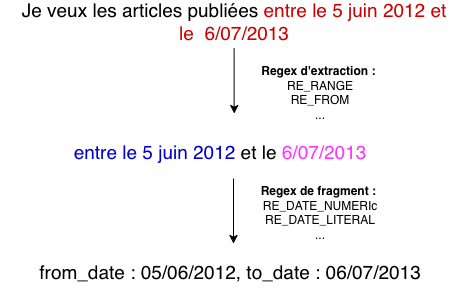
\includegraphics[width=0.4\textwidth]{assets/dateextractor.drawio.png}
    \caption{Extraction des dates}
    \label{fig:dateextractor}
\end{figure}
>>>>>>> rapport

\section{Extraction des mots clés}
Une des plus grandes difficultés a été l'extraction des mots clés, car il y a beaucoup de variabilité dans les requêtes. La classe en charge de cette partie est \texttt{KeyWordExtractor}. Pour cette partie, il a fallu déterminer une liste de stop words propres aux requêtes, car par exemple "je" et "veux" ne sont peut-être pas des stop words du corpus, mais dans les requêtes ils ne sont pas importants. 

Pour extraire les mots clé, il faut d'abord extraire les parties de la requête les contenant. \texttt{RE\_TITRE} et \texttt{RE\_CONTENU} permettent de distinguer les mots clés du titre et du contenu, il y a aussi d'autres regex pour des cas particuliers.
Une fois ces bouts de texte extraits, ils sont traités par la méthode \texttt{\_parse\_logic\_block()} qui construit le DNF pour les mots clés. Elle détecte les opérateurs de conjonction via des regex et sépare le texte logiquement. Si le mot n'est pas un stop word ni du corpus ni des requêtes, alors il est lemmatisé et corrigé par \texttt{normalize\_terms()}.


\section{Classe Pretraiteur}

La classe \texttt{Pretraiteur} encapsule tout le pipeline pour passer d'une requête brute à une requête formatée. Elle utilise les classes \texttt{DateExtractor} et \texttt{KeyWordExtractor} pour extraire les dates et les mots clés. Pour les traitements plus simples (bulletin, image ou non, etc.), la logique est directement mise dans des méthodes de \texttt{Pretraiteur}. 
<<<<<<< HEAD
C'est la méthode \texttt{treat\_request()} qui effectue la totalité du pipeline. Chaque traitement retire la partie traitée, ce qui permet d'éviter les conflits.

\begin{figure}[h]
    \centering
    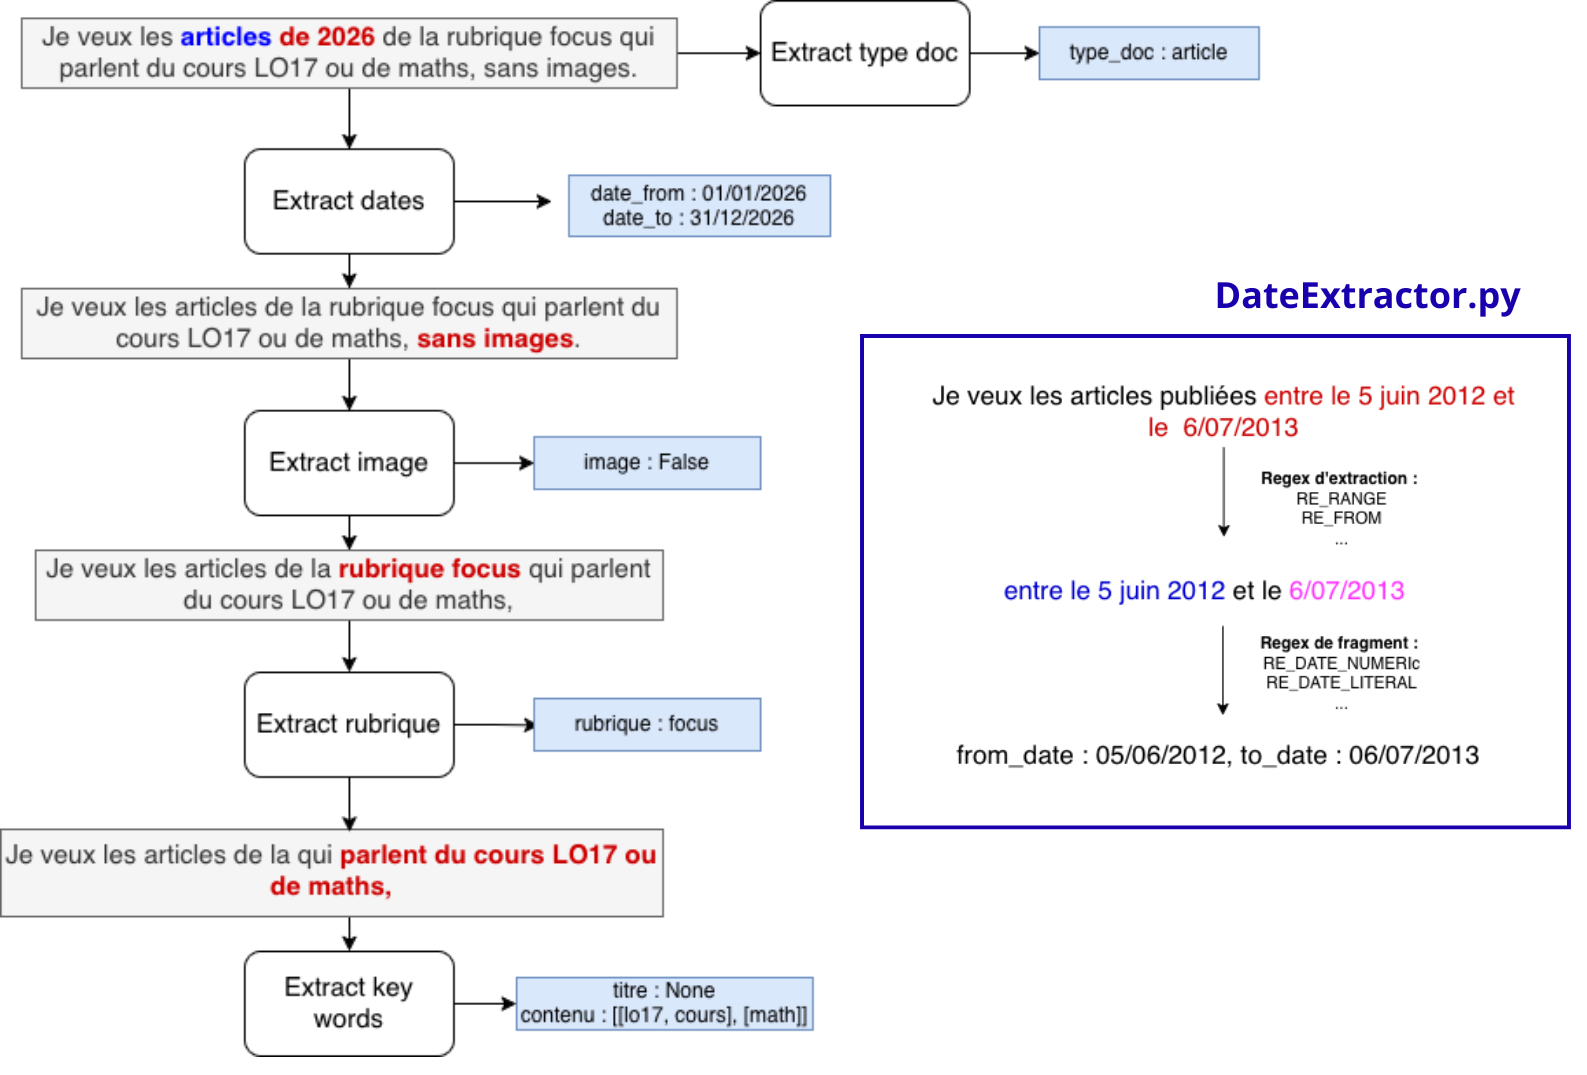
\includegraphics[width=0.8\textwidth]{assets/pretraiteur.png}
    \caption{Pipeline de traitement des requêtes (Pretraiteur + DateExtractor)}
    \label{fig:pretraiteur}
\end{figure}

\begin{figure}[h]
    \centering
    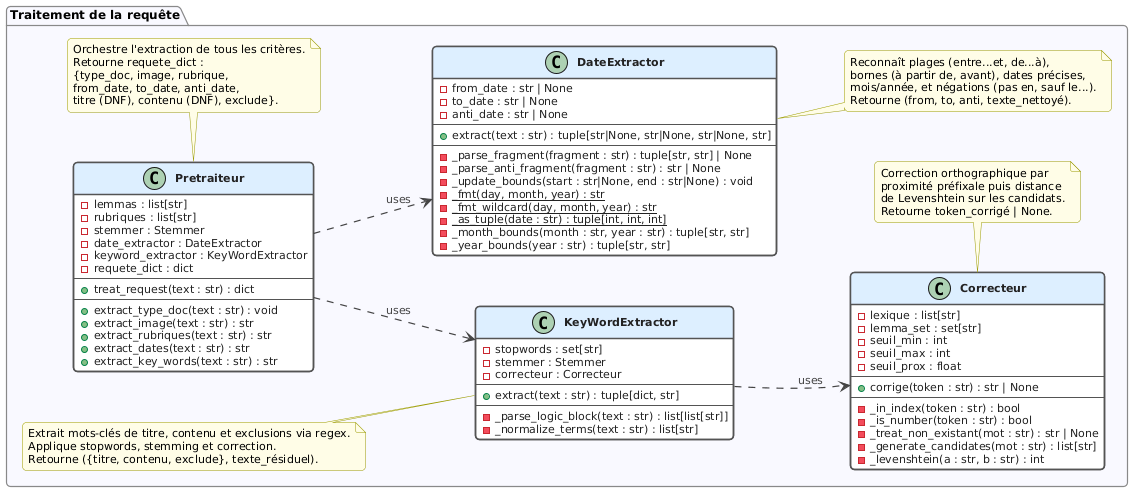
\includegraphics[width=1.1\textwidth]{assets/3-pretraiteur.png}
    \caption{UML Pretraiteur + Correcteur (TD4 et TD5)}
    \label{fig:UMLpretraiteur}
=======
C'est la méthode \texttt{treat\_request()} qui effectue la totalité du pipeline. Chaque traitement retire la partie traitée, ce qui permet d'éviter les conflits. La figure \ref{fig:pretraiteur} décrit les étapes du pipeline de formatage.

\begin{figure}[h]
    \centering
    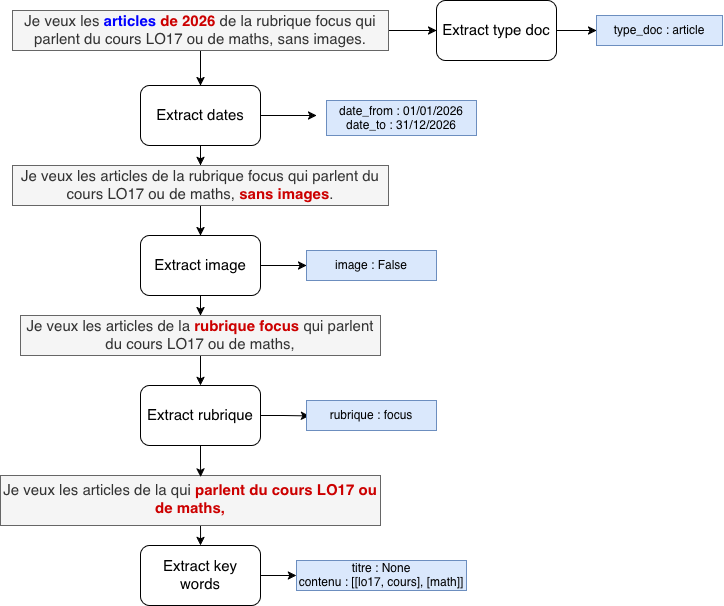
\includegraphics[width=0.6\textwidth]{assets/pretraiteur.drawio.png}
    \caption{Pipeline de traitement des requêtes (Pretraiteur)}
    \label{fig:pretraiteur}
>>>>>>> rapport
\end{figure}